\documentclass[11pt]{amsart}
\usepackage[margin=1.1in]{geometry}
\usepackage{amssymb,mathtools}
\usepackage{graphicx}
\usepackage[hidelinks]{hyperref}
\usepackage{doi}

\newcommand{\zenodoDOI}{10.5281/zenodo.24123896}

\newtheorem{theorem}{Theorem}[section]
\newtheorem{lemma}[theorem]{Lemma}
\newtheorem{proposition}[theorem]{Proposition}
\newtheorem{corollary}[theorem]{Corollary}
\newtheorem*{theoremA}{Theorem A}
\newtheorem*{corollaryB}{Corollary B}
\theoremstyle{definition}
\newtheorem{definition}[theorem]{Definition}
\theoremstyle{remark}
\newtheorem{remark}[theorem]{Remark}
\newtheorem{example}[theorem]{Example}

\newcommand{\Z}{\mathbb{Z}}
\newcommand{\cV}{\mathcal{V}}
\newcommand{\cR}{\mathcal{R}}
\newcommand{\cW}{\mathcal{W}}
\newcommand{\Stab}{\mathcal{S}}
\newcommand{\stab}{\operatorname{stab}}
\newcommand{\supp}{\operatorname{supp}}
\newcommand{\ket}[1]{|#1\rangle}
\newcommand{\two}{\mathbf{2}}
\newcommand{\one}{\mathbf{1}}
\newcommand{\Ind}[1]{[\,#1\,]}

\begin{document}

\title{The Oslo Rice Pile Relaxes Exactly in $L(L+1)$ Steps}

\author{Deep Bhattacharjee}
\address{Formerly, Electro-Gravitational Space Propulsion Laboratory (EGSPL), Bhubaneswar, Odisha 751030, India}
\address{Formerly, University of Calcutta (Heramba Chandra College), 23/49 Gariahat Road, Golpark, Kolkata 700029, West Bengal, India}
\email{d.bhattacharjee@erl-forschung.de}
\email{itsdeep@live.com}
\email{egspl@proton.me (GitHub-related contact; GitHub: creelie)}
\urladdr{https://orcid.org/0000-0003-0466-750X}

\subjclass[2020]{60J10, 82C20, 05C57}
\keywords{Oslo model, abelian sandpile, chip-firing}

\begin{abstract}
Dhar stated that the evolution operator $\cW$ of the Oslo rice pile on $L$ sites satisfies $\cW^{n+1}=\cW^n$ with $n=L(L+1)/2$. This is false: the least such $n$ is $L(L+1)$. We prove that a configuration $\sigma$ with $g$ grains reaches the steady state after exactly $L(L+1)-g+\Ind{\sigma_L=2}$ added grains, and that Dhar's decorrelation time $L(L+1)/2$ is nevertheless exact on recurrent configurations.
\end{abstract}

\maketitle

\section{Introduction}

The Oslo rice pile \cite{CCFFJ96,FCMFJM96} is a one-dimensional sandpile in which the critical slope of a site is drawn afresh, equal to $1$ with probability $q$ and to $2$ with probability $p=1-q$, each time the site topples. It is driven by dropping grains at the top of the pile and has been studied as a model of self-organized criticality \cite{BTW87,Pru12} and of interface depinning \cite{PB96,Pru03,GDM16}. In \cite{Dha04} Dhar showed that, in slope variables, the model is an abelian distributed processors network \cite{Dha99}, a stochastic relative of the abelian sandpile \cite{Dha90}, wrote down the operators $a_1,\dots,a_L$ that add a particle at a site and relax, and drew strong conclusions about the evolution operator $\cW=a_1$ acting on the $3^L$-dimensional space $\cV$ spanned by the stable configurations. The abstract of \cite{Dha04} reads, in part: ``We show that the time evolution operator $\cW$ for the system satisfies the equation $\cW^{n+1}=\cW^n$ where $n=L(L+1)/2$ for a pile with $L$ sites.''

This identity is false for every $L\ge1$. For $L=1$ it would say $\cW^2=\cW$, but $\cW\ket{0}=\ket{1}$ while $\cW^2\ket{0}=p\ket{2}+q\ket{1}$. The body of \cite{Dha04} proves the weaker identity $\cW^{L(L+1)+1}=\cW^{L(L+1)}$ and then states, for every recurrent configuration $\mathcal C$ with $m$ grains,
\begin{equation}\label{eq:dharlemma}
a_1^{L(L+1)-m}\ket{\mathcal C}=a_1^2a_2^2\cdots a_L^2\ket{0,\dots,0},
\end{equation}
from which it deduces that $\cW^{L(L+1)/2}$ sends every recurrent configuration to the steady state $\ket{\Psi}$ and that every connected time-dependent correlation function vanishes beyond time difference $L(L+1)/2$. The configuration $\mathcal C=(2,\dots,2)$ is recurrent and has $m=L(L+1)$ grains, so \eqref{eq:dharlemma} would give $\ket{2,\dots,2}=\ket{\Psi}$, which is false because $\Psi$ also charges $(1,\dots,1)$ (Proposition~\ref{prop:rec}). The present paper determines the exact relaxation time of every configuration and thereby settles which of the statements of \cite{Dha04} hold.

Throughout, $L\ge1$ and $0<p<1$. A stable configuration is a vector $\sigma=(\sigma_1,\dots,\sigma_L)\in\{0,1,2\}^L$ of slopes. Its number of grains is\footnote{If $h_x$ is the height of column $x$ and $h_{L+1}=0$, then $\sigma_x=h_x-h_{x+1}$ and $\sum_x h_x=\sum_x\sum_{y\ge x}\sigma_y=\sum_y y\,\sigma_y$.}
\[
g(\sigma)=\sum_{x=1}^L x\,\sigma_x .
\]
Let $r(\sigma)$ be the length of the longest block of $2$'s ending at site $L$, so that $r(\sigma)=0$ when $\sigma_L\ne2$, and write $\two=(2,\dots,2)$, $\one=(1,\dots,1)$ and $u=(1,2,\dots,2)$. The vector $v_u=a_1a_2^2\cdots a_L^2\ket{0}$ is the law of the pile obtained from the empty pile by adding one particle at site $1$ and two at each other site.

\begin{theoremA}
For every stable configuration $\sigma$ and every $k\ge0$,
\[
\cW^k\ket{\sigma}=\ket{\Psi}\iff k\ge K(\sigma),\qquad K(\sigma)=L(L+1)-g(\sigma)+\Ind{\sigma_L=2}.
\]
Moreover $K(\sigma)\ge1$, and with $r=r(\sigma)$,
\[
\cW^{K(\sigma)-1}\ket{\sigma}=
\begin{cases}
v_u, & r=0,\\[2pt]
p^{-r}\ket{\Psi}+\bigl(1-p^{-r}\bigr)v_u, & r\ge1.
\end{cases}
\]
\end{theoremA}

The second statement shows exactly what goes wrong one step before relaxation: when the last slope is $2$, the steady state appears with weight $p^{-r}>1$, compensated by the negative weight $1-p^{-r}$ of a vector that has not yet reached the top configuration $\two$. The recurrent configurations are those charged by $\Psi$; they are described in Section~\ref{sec:recurrent}.

\begin{corollaryB}
\begin{enumerate}
\item The least $n$ with $\cW^{n+1}=\cW^n$ on $\cV$ is $L(L+1)$, and $\ket{0,\dots,0}$ is the only configuration that needs $L(L+1)$ grains. The minimal polynomial of $\cW$ is $x^{L(L+1)}(x-1)$, so $\cW$ has a nilpotent Jordan block of size $L(L+1)$.
\item On the span $\cV_{\mathrm{rec}}$ of the recurrent configurations the least such $n$ is $L(L+1)/2$, and the minimal polynomial of $\cW|_{\cV_{\mathrm{rec}}}$ is $x^{L(L+1)/2}(x-1)$.
\item In the steady state every connected correlation $C_{XY}(\tau)$ vanishes for $\tau\ge L(L+1)/2$, and there are observables with $C_{XY}(L(L+1)/2-1)<0$.
\item Identity \eqref{eq:dharlemma} holds for every configuration $\mathcal C$ with $\mathcal C_L\ne2$, recurrent or not, and fails for every configuration with $\mathcal C_L=2$; recurrent configurations with $\mathcal C_L=2$ exist for every $L$.
\end{enumerate}
\end{corollaryB}

So the statement in the abstract of \cite{Dha04} is true on $\cV_{\mathrm{rec}}$ and false on $\cV$, the identity in its body is optimal, and its physical conclusions about correlations are correct and sharp; what fails is \eqref{eq:dharlemma} and the operator identity as stated. The proofs are self-contained. Section~\ref{sec:model} sets up the model and its abelian property, Section~\ref{sec:chip} reduces products of the operators $a_x$ to a deterministic chip-firing game, Section~\ref{sec:expansion} expands every configuration in the vectors $a^m\ket{0}$, Section~\ref{sec:proofA} proves Theorem~A, Section~\ref{sec:recurrent} describes the recurrent configurations, and Section~\ref{sec:proofB} proves Corollary~B. Figure~\ref{fig:K} shows $K(\sigma)$ for all configurations at $L=5$.

\begin{figure}[t]
\centering
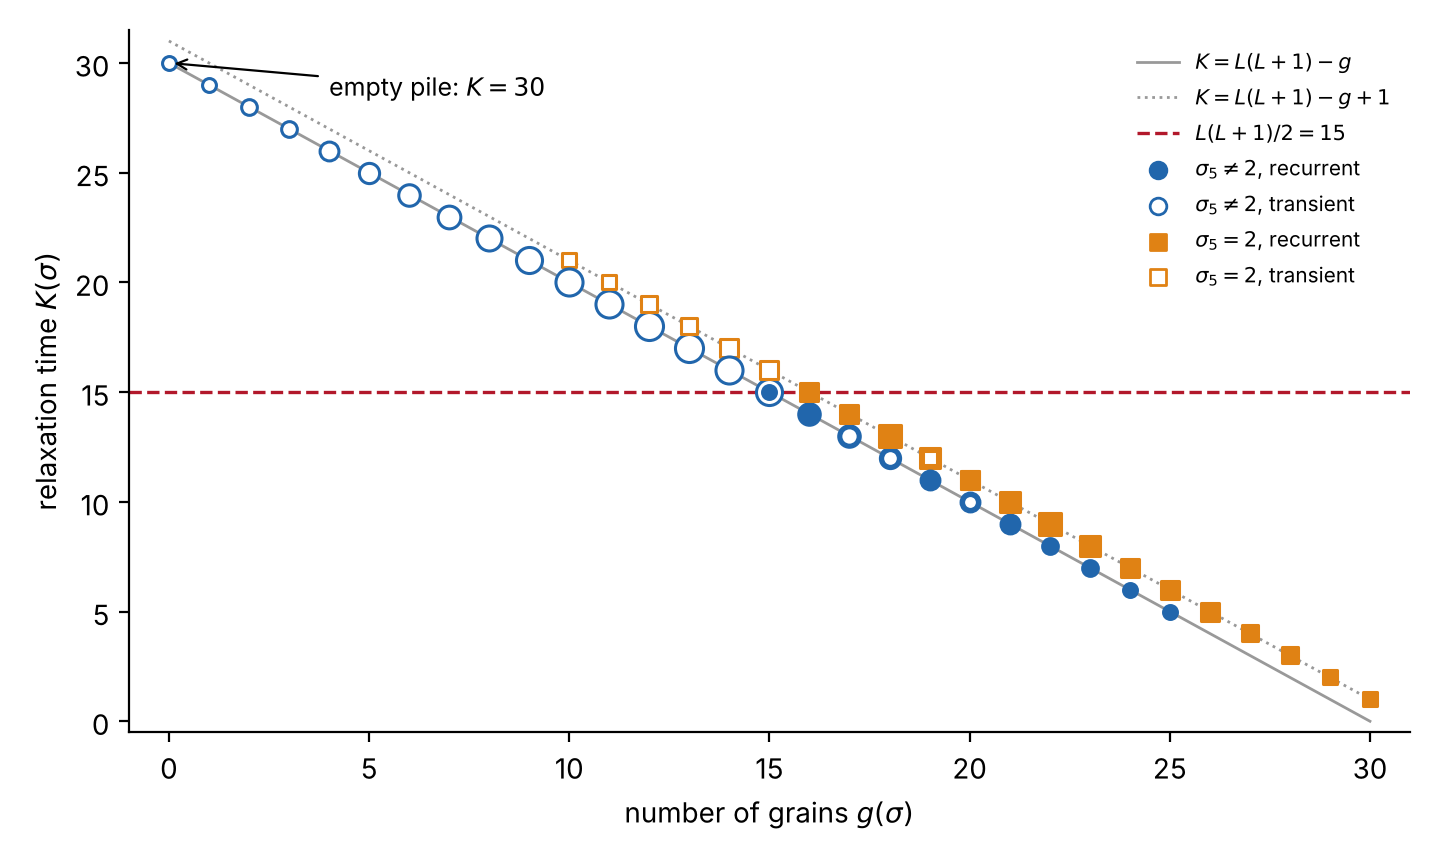
\includegraphics[width=0.82\textwidth]{fig_relaxation.png}
\caption{The relaxation time $K(\sigma)$ against the number of grains $g(\sigma)$ for all $3^5$ configurations at $L=5$. Configurations with $\sigma_5=2$ lie one step above the line $K=30-g$. Filled marks are recurrent; all of them lie on or below the dashed level $L(L+1)/2=15$, which is attained. The empty pile alone needs $L(L+1)=30$ grains, whereas the abstract of \cite{Dha04} asserts $15$ for every configuration. Mark size grows with the number of configurations at a point; a filled mark inside an open one means that both recurrent and transient configurations occur there.}
\label{fig:K}
\end{figure}

\section{The model and its abelian property}\label{sec:model}

\subsection{Particles}
Following \cite[Sections~3--4]{Dha04} we describe the pile by its slopes and call the units of slope particles. Adding a grain at the top raises $\sigma_1$ by one, that is, it adds a particle at site $1$. When a particle arrives at a site $x$ in state $\sigma_x$:
\begin{itemize}
\item if $\sigma_x=0$, then $\sigma_x$ becomes $1$;
\item if $\sigma_x=1$, then with probability $p$ the slope becomes $2$, and with probability $q$ the site topples: $\sigma_x$ becomes $0$ and one particle is sent to each of $x-1$ and $x+1$;
\item if $\sigma_x=2$, the site topples: $\sigma_x$ becomes $1$ and one particle is sent to each of $x-1$ and $x+1$.
\end{itemize}
A particle sent to site $0$ leaves the system, and a particle sent to site $L+1$ is delivered to site $L$.\footnote{A toppling at $x<L$ moves one grain from column $x$ to column $x+1$. A toppling at $L$, followed by the arrival of the particle sent back to $L$, changes $(\sigma_{L-1},\sigma_L)$ by $(+1,-1)$, which is rule (ii)c of \cite{Dha04}: one grain leaves the pile.} This is the rule by which Dhar replaces the critical thresholds \cite[Section~3]{Dha04}.\footnote{In the threshold description, from the toppling of $x$ that draws a threshold until the next arrival at slope $1$, the slope of $x$ stays at most $1$, so the threshold has not been tested and is still distributed as a fresh draw at that arrival; a site at slope $2$ has threshold $2$. Processing one particle at a time, the two descriptions therefore give the same process.} The operators of \cite{Dha04}, and hence all its statements, refer to this process.

To make the randomness explicit, give every site $x$ an infinite sequence $\xi_x=(\xi_x(1),\xi_x(2),\dots)$ of symbols in $\{\mathsf S,\mathsf T\}$ (stay, topple). When a particle arrives at $x$ while $\sigma_x=1$, the site reads the next unread symbol of $\xi_x$ and stays at $2$ on $\mathsf S$ or topples on $\mathsf T$. When the sequences are independent with independent entries, each equal to $\mathsf S$ with probability $p$, this reproduces the rule above.

A \emph{state} consists of a configuration $\sigma\in\Z_{\ge0}^L$ (not necessarily stable during relaxation), a vector $\eta\in\Z_{\ge0}^L$ of pending particles, and the number of symbols read at each site. A \emph{step} chooses a site $x$ with $\eta_x\ge1$ and processes one of its pending particles. Starting from a stable $\sigma$ and an input $\lambda\in\Z_{\ge0}^L$, with $\eta=\lambda$ initially, a \emph{relaxation} is a sequence of steps; it is \emph{complete} if it ends with $\eta=0$. The relaxation of a single particle at a stable site always ends in a stable slope, so a complete relaxation ends in a stable configuration.

Throughout we use $e_x$ for the unit vector at $x$, together with the conventions
\[
e_0=0,\qquad e_{L+1}=e_L,
\]
and the $L\times L$ matrix $D$ with columns $De_x=2e_x-e_{x-1}-e_{x+1}$; explicitly $D$ is tridiagonal with diagonal $(2,\dots,2,1)$ and off-diagonal entries $-1$.\footnote{For $x=L$ the convention gives $De_L=e_L-e_{L-1}$.} Its inverse is
\begin{equation}\label{eq:Dinv}
D^{-1}=\bigl(\min(x,y)\bigr)_{x,y=1}^L ,
\end{equation}
as one checks column by column: for $x<L$, $2\min(x,y)-\min(x-1,y)-\min(x+1,y)=\delta_{xy}$, and $\min(L,y)-\min(L-1,y)=\delta_{Ly}$. In particular $D^{-1}$ has nonnegative entries. The \emph{weight} of a vector $m\in\Z^L$ is $w(m)=\sum_x x\,m_x$; thus $g(\sigma)=w(\sigma)$. Since $\sum_x x\,D_{xy}=0$ for $y<L$ and $=1$ for $y=L$,
\begin{equation}\label{eq:weightD}
w(m-Df)=w(m)-f_L\qquad(m,f\in\Z^L).
\end{equation}

\subsection{The effective configuration}
Along a relaxation put $\tilde\sigma=\sigma+\eta$. A step that does not topple moves one particle from $\eta_x$ to $\sigma_x$ and leaves $\tilde\sigma$ unchanged. A toppling at $x$ lowers $\sigma_x+\eta_x$ by $2$ and sends one particle to each of $x\pm1$ under the conventions above, so it replaces $\tilde\sigma$ by $\tilde\sigma-De_x$. A toppling at $x$ requires $\sigma_x\ge1$ and $\eta_x\ge1$, so $\tilde\sigma_x\ge2$; if it happens at $\sigma_x=2$ then $\tilde\sigma_x\ge3$.

\begin{lemma}\label{lem:term}
Let $\sigma$ be stable and $\lambda\in\Z_{\ge0}^L$. Every relaxation from $(\sigma,\lambda)$ has at most
\[
M(\sigma,\lambda)=|\lambda|+2\sum_{x=1}^L\bigl(D^{-1}(\sigma+\lambda)\bigr)_x
\]
steps, where $|\lambda|=\sum_x \lambda_x$. In particular every relaxation can be continued to a complete one.
\end{lemma}

\begin{proof}
Let $N\in\Z_{\ge0}^L$ count the topplings so far. Then $\tilde\sigma=\sigma+\lambda-DN\ge0$, so $DN\le\sigma+\lambda$ and, $D^{-1}$ being nonnegative, $N\le D^{-1}(\sigma+\lambda)$. Each step processes a particle that was either in the input or sent by one of the topplings, and each toppling sends at most two particles. Hence the number of steps is at most $|\lambda|+2\sum_xN_x\le M(\sigma,\lambda)$. As long as $\eta\ne0$ a further step is possible, so the bound forces every relaxation to reach $\eta=0$ if continued.
\end{proof}

\begin{lemma}\label{lem:unique}
Fix the sequences $\xi$, a stable $\sigma$ and an input $\lambda$. All complete relaxations from $(\sigma,\lambda)$ process the same number of particles at each site and end in the same state.
\end{lemma}

\begin{proof}
Given $\sigma_x$ and $\xi_x$, the behaviour of site $x$ depends only on the number $n_x$ of particles it has processed: its slope, the number of symbols it has read and the number $c_x(n_x)$ of its topplings are functions of $n_x$, and $c_x$ is nondecreasing. Put $c_0=c_{L+1}=0$. When $n\in\Z_{\ge0}^L$ particles have been processed, the number of pending particles at $x$ is
\[
\eta_x(n)=\lambda_x+c_{x-1}(n_{x-1})+c_{x+1}(n_{x+1})+\Ind{x=L}\,c_L(n_L)-n_x .
\]
For $y\ne x$ this is nondecreasing in $n_y$. Let $\alpha$ and $\beta$ be complete relaxations with final counts $n^\alpha$ and $n^\beta$, so $\eta(n^\beta)=0$. Suppose some step of $\alpha$ processes a particle at a site $x$ that has already processed $n^\beta_x$ particles in $\alpha$, and take the first such step. Just before it the counts $n$ satisfy $n\le n^\beta$ and $n_x=n^\beta_x$, hence $\eta_x(n)\le\eta_x(n^\beta)=0$, and the step is impossible. Thus $n^\alpha\le n^\beta$, and by symmetry $n^\alpha=n^\beta$. The final state is a function of the counts.
\end{proof}

\subsection{The operators}
For a stable $\sigma$ and an input $\lambda$ let $\Phi(\sigma,\lambda;\xi)$ be the final configuration of any complete relaxation, and let $P_\lambda$ be the linear operator on $\cV$ with
\[
P_\lambda\ket{\sigma}=\sum_{\sigma'}\Pr\bigl(\Phi(\sigma,\lambda;\xi)=\sigma'\bigr)\ket{\sigma'} ,
\]
the sequences $\xi$ being random as above. Only finitely many symbols are read (Lemma~\ref{lem:term}), so these probabilities are well defined. Put $a_x=P_{e_x}$ for $1\le x\le L$, $a_0=1$ and $a_{L+1}=a_L$. Then $\cW=a_1$ is the transition matrix of the driven pile, and $\cW$ maps probability vectors to probability vectors.

\begin{proposition}\label{prop:compose}
For inputs $\lambda,\lambda'$ we have $P_{\lambda+\lambda'}=P_{\lambda'}P_\lambda$. Consequently the $a_x$ commute and $P_\lambda=\prod_x a_x^{\lambda_x}$.
\end{proposition}

\begin{proof}
Relax $(\sigma,\lambda+\lambda')$ in two phases. In the first, process only the particles of $\lambda$ and those they generate, exactly as in a complete relaxation of $(\sigma,\lambda)$; this is a legitimate sequence of steps because the extra pending particles $\lambda'$ only enlarge $\eta$. Then complete the relaxation. By Lemma~\ref{lem:unique} the result is $\Phi(\sigma,\lambda+\lambda';\xi)$. Run the first phase by a fixed rule (always the smallest site with a pending particle of the first phase). Whether it ends in the configuration $\sigma''$ after reading $k_x$ symbols at each $x$ is decided by the first $k_x$ symbols of each $\xi_x$. Conditionally on this event, the unread parts $(\xi_x(k_x+1),\xi_x(k_x+2),\dots)$ are again independent with independent entries of the same law, and the second phase is a complete relaxation of $(\sigma'',\lambda')$ driven by them. Summing over the events gives $P_{\lambda+\lambda'}\ket\sigma=P_{\lambda'}P_\lambda\ket\sigma$. Since $\lambda+\lambda'=\lambda'+\lambda$, the operators $P_\lambda$ commute, and induction on $|\lambda|$ gives $P_\lambda=\prod_xa_x^{\lambda_x}$.
\end{proof}

\begin{proposition}[Dhar's relations]\label{prop:relations}
Let $\sigma$ be stable and $1\le x\le L$. Then
\begin{align}
a_x\ket{\sigma}&=\ket{\sigma+e_x} &&\text{if }\sigma_x=0, \tag{R0}\label{R0}\\
a_x\ket{\sigma}&=p\ket{\sigma+e_x}+q\,a_{x-1}a_{x+1}\ket{\sigma-e_x} &&\text{if }\sigma_x=1, \tag{R1}\label{R1}\\
a_x\ket{\sigma}&=a_{x-1}a_{x+1}\ket{\sigma-e_x} &&\text{if }\sigma_x=2. \tag{R2}\label{R2}
\end{align}
\end{proposition}

\begin{proof}
Process the added particle first. If $\sigma_x=0$ the configuration $\sigma+e_x$ is stable. If $\sigma_x=1$ the first symbol of $\xi_x$ is $\mathsf S$ with probability $p$, giving the stable $\sigma+e_x$; otherwise the site falls to $0$ and sends particles to $x\pm1$. If $\sigma_x=2$ it falls to $1$ and sends particles to $x\pm1$. In the toppling cases the remaining relaxation is a complete relaxation of $\sigma-e_x$ with input $e_{x-1}+e_{x+1}$, driven by the unread symbols, which are independent of the first one; by the argument of Proposition~\ref{prop:compose} its law is $P_{e_{x-1}+e_{x+1}}\ket{\sigma-e_x}=a_{x-1}a_{x+1}\ket{\sigma-e_x}$, with $e_0=0$, $e_{L+1}=e_L$.
\end{proof}

\section{Monomials and chip-firing}\label{sec:chip}

For $m\in\Z_{\ge0}^L$ write $a^m=a_1^{m_1}\cdots a_L^{m_L}$ and $v_m=a^m\ket{0}$, where $\ket{0}=\ket{0,\dots,0}$. By Proposition~\ref{prop:compose}, $v_m=P_m\ket0$ is a probability vector.

\begin{lemma}\label{lem:cube}
$a_x^3=a_{x-1}a_xa_{x+1}$ for $1\le x\le L$.
\end{lemma}

\begin{proof}
We check the identity on each basis vector, using commutativity and \eqref{R0}--\eqref{R2}. Write $\ket{j}$ for $\ket{\sigma}$ with $\sigma_x=j$ and the other slopes fixed, and $b=a_{x-1}a_{x+1}$. First, $a_x^2\ket1=a_x(p\ket2+qb\ket0)=pb\ket1+qb\,a_x\ket0=b\ket1$. Hence
\begin{gather*}
a_x^3\ket0=a_x^2\ket1=b\ket1=b\,a_x\ket0,\qquad
a_x^3\ket1=a_xb\ket1=b\,a_x\ket1,\\
a_x^3\ket2=a_x^2b\ket1=b\,a_x^2\ket1=b\,b\ket1=b\,a_x\ket2 .\qedhere
\end{gather*}
\end{proof}

Call $x$ \emph{unstable} in $m\in\Z_{\ge0}^L$ if $m_x\ge3$; \emph{firing} $x$ replaces $m$ by $m-De_x$, that is, $m_x$ drops by $2$ and each of $x\pm1$ gains $1$ (so $m_L$ drops by $1$ when $x=L$, and nothing is added at site $0$). A firing is \emph{legal} if $x$ is unstable. A vector is \emph{stable} if $m\le\two$ entrywise, and these are exactly the stable configurations. By Lemma~\ref{lem:cube}, if $m_x\ge3$ then
\begin{equation}\label{eq:firing}
a^m=a^{m-3e_x}a_x^3=a^{m-3e_x}a_{x-1}a_xa_{x+1}=a^{m-De_x}.
\end{equation}

\begin{lemma}[least action]\label{lem:LAP}
Let $m\in\Z_{\ge0}^L$ and $f\in\Z_{\ge0}^L$ with $(m-Df)_x\le2$ for every $x$. Then every sequence of legal firings starting at $m$ fires each $x$ at most $f_x$ times.
\end{lemma}

\begin{proof}
Suppose not, and consider the first firing in the sequence that fires some $x$ for the $(f_x+1)$-st time. Just before it the firing counts $F$ satisfy $F\le f$ and $F_x=f_x$. The off-diagonal entries of $D$ are $\le0$, so
\[
(m-DF)_x=m_x-D_{xx}f_x-\sum_{y\ne x}D_{xy}F_y\le m_x-D_{xx}f_x-\sum_{y\ne x}D_{xy}f_y=(m-Df)_x\le2,
\]
and $x$ is not unstable, a contradiction.
\end{proof}

This principle is due to Fey, Levine and Peres \cite{FLP10} for the abelian sandpile; the proof above is theirs, adapted to the matrix $D$.

\begin{corollary}\label{cor:stab}
Every sequence of legal firings from $m$ is finite, and all maximal sequences have the same firing vector $F(m)$ and end in the same stable vector $\stab(m)=m-DF(m)$. Moreover:
\begin{enumerate}
\item $a^m=a^{\stab(m)}$ and $v_m=v_{\stab(m)}$;
\item $w(\stab(m))=w(m)-F_L(m)$;
\item $\stab(m+m')=\stab(\stab(m)+m')$ for $m'\in\Z_{\ge0}^L$.
\end{enumerate}
\end{corollary}

\begin{proof}
Along legal firings the vector stays nonnegative, so the firing vector $F$ satisfies $DF\le m$ and hence $F\le D^{-1}m$ by \eqref{eq:Dinv}; every sequence is therefore finite. If $\alpha,\beta$ are maximal, the end vector $m-DF^\beta$ of $\beta$ is stable, so Lemma~\ref{lem:LAP} with $f=F^\beta$ gives $F^\alpha\le F^\beta$, and symmetry gives equality. Item (1) follows from \eqref{eq:firing}, item (2) from \eqref{eq:weightD}. For (3), a maximal sequence for $m$ remains legal from $m+m'$, since adding chips never makes a firing illegal; continuing it maximally stabilizes $\stab(m)+m'$, and the result is $\stab(m+m')$ by uniqueness.
\end{proof}

The stable vectors have weight at most $w(\two)=L(L+1)$, with equality only for $\two$, and $\two-e_1=u$ is the only stable vector of weight $L(L+1)-1$.\footnote{If $s\le\two$ then $w(\two)-w(s)=\sum_xx(2-s_x)$ is a sum of nonnegative terms, which equals $1$ only for $2-s=e_1$.}

\begin{lemma}\label{lem:addone}
Let $s$ be stable. If $s\ne\two$, then $\stab(s+e_1)$ has weight $w(s)+1$ and site $L$ does not fire. If $s=\two$, then $\stab(\two+e_1)=\two$.
\end{lemma}

\begin{proof}
If $s\ne\two$, let $j$ be the least site with $s_j\le1$. If $j=1$ nothing fires. Otherwise fire $1,2,\dots,j-1$ in this order. Before the firing of $i\le j-1$ the vector is $(2,\dots,2,1,3,2,\dots)$ with the $3$ at position $i$ (for $i=1$, simply $3$ at position $1$), so the firing is legal; after it the vector is $(2,\dots,2,1,3,\dots)$ with the $1$ at position $i$ and the $3$ moved to $i+1$, except that after firing $j-1$ the entry at $j$ is $s_j+1\le2$. The final vector is stable, no firing occurred at $L$ because $j-1<L$, and by Corollary~\ref{cor:stab}(2) the weight rose by $1$. If $s=\two$, the same sequence fires $1,\dots,L-1$ and produces $(2,\dots,2,1,3)$; firing $L$ then gives $\two$. (For $L=1$, the vector $3$ fires once to $2$.)
\end{proof}

\begin{corollary}\label{cor:climb}
Let $s$ be stable and $k\ge0$. If $k\ge L(L+1)-w(s)$ then $\stab(s+ke_1)=\two$. If $k<L(L+1)-w(s)$ then $\stab(s+ke_1)$ is stable of weight $w(s)+k$. In particular $\stab(L(L+1)e_1)=\two$.
\end{corollary}

\begin{proof}
By Corollary~\ref{cor:stab}(3), $\stab(s+(k+1)e_1)=\stab(\stab(s+ke_1)+e_1)$. By Lemma~\ref{lem:addone} each added chip raises the weight by exactly one until the weight $L(L+1)$, that is the vector $\two$, is reached, and $\two$ is then fixed.
\end{proof}

\section{Expansion of a configuration and the steady state}\label{sec:expansion}

\begin{lemma}\label{lem:expansion}
Let $\sigma$ be stable and $T=\{x:\sigma_x=2\}$, $t=|T|$. For $A\subseteq T$ put $\tau_A=\sigma-D\mathbf 1_A$, where $\mathbf 1_A=\sum_{x\in A}e_x$. Then $\tau_A\ge0$ and
\[
\ket\sigma=p^{-t}\sum_{A\subseteq T}(-q)^{|A|}\,v_{\tau_A}.
\]
\end{lemma}

\begin{proof}
By \eqref{R0}, $a_x\ket{\rho}=\ket{\rho+e_x}$ when $\rho_x=0$; and by \eqref{R0}--\eqref{R1}, $a_x^2\ket{\rho}=a_x\ket{\rho+e_x}=p\ket{\rho+2e_x}+q\,a_{x-1}a_{x+1}\ket\rho$ when $\rho_x=0$, that is
\begin{equation}\label{eq:two}
\ket{\rho+2e_x}=p^{-1}\bigl(a_x^2-q\,a_{x-1}a_{x+1}\bigr)\ket\rho\qquad(\rho\text{ stable},\ \rho_x=0).
\end{equation}
Let $\sigma^\circ$ be $\sigma$ with every $2$ replaced by $0$; then $\ket{\sigma^\circ}=a^{\sigma^\circ}\ket0$ by repeated use of \eqref{R0}. Applying \eqref{eq:two} once for each $x\in T$ and using commutativity,
\[
\ket\sigma=p^{-t}\prod_{x\in T}\bigl(a_x^2-q\,a_{x-1}a_{x+1}\bigr)a^{\sigma^\circ}\ket0=p^{-t}\sum_{A\subseteq T}(-q)^{|A|}a^{\tau_A}\ket0,
\]
because the monomial chosen from the factors is $a^{\sigma^\circ}\prod_{x\in T\setminus A}a_x^2\prod_{x\in A}a_{x-1}a_{x+1}$, whose exponent is $\sigma^\circ+2\mathbf 1_{T\setminus A}+\sum_{x\in A}(e_{x-1}+e_{x+1})=\sigma-D\mathbf 1_A$.
\end{proof}

By Corollary~\ref{cor:stab}(2) and \eqref{eq:weightD}, $w(\tau_A)=g(\sigma)-\Ind{L\in A}$, and
\begin{equation}\label{eq:sA}
s_A:=\stab(\tau_A)\quad\text{has weight}\quad w(s_A)=g(\sigma)-\mu_A,\qquad \mu_A:=\Ind{L\in A}+F_L(\tau_A).
\end{equation}

Define the steady state by $\ket\Psi=v_\two=a_1^2a_2^2\cdots a_L^2\ket0$.

\begin{lemma}\label{lem:Psi}
$\ket\Psi=\cW^{L(L+1)}\ket0=a_1\ket\two$ and $\cW\ket\Psi=\ket\Psi$.
\end{lemma}

\begin{proof}
By Corollaries~\ref{cor:stab}(1) and \ref{cor:climb}, $\cW^{L(L+1)}\ket0=v_{L(L+1)e_1}=v_\two$ and $\cW\ket\Psi=v_{\two+e_1}=v_\two$. For the remaining identity, if $\rho_x=2$ then by \eqref{R2}, commutativity and \eqref{R0}--\eqref{R1},
\[
a_x^3\ket{\rho-2e_x}=a_x^2\ket{\rho-e_x}=a_x\bigl(p\ket\rho+q\,a_{x-1}a_{x+1}\ket{\rho-2e_x}\bigr)=p\,a_x\ket\rho+q\,a_{x-1}a_{x+1}\ket{\rho-e_x}=a_x\ket\rho .
\]
Let $\rho^{(j)}=(0,\dots,0,2,\dots,2)$ with $j-1$ zeros. We claim $a_1\ket\two=a_1^2\cdots a_{j-2}^2\,a_{j-1}a_j\ket{\rho^{(j)}}$ for $1\le j\le L+1$ (for $j=1$ the right side is $a_0a_1\ket\two$). Given the claim for $j\le L$, the displayed identity and Lemma~\ref{lem:cube} give $a_j\ket{\rho^{(j)}}=a_j^3\ket{\rho^{(j+1)}}=a_{j-1}a_ja_{j+1}\ket{\rho^{(j+1)}}$, which is the claim for $j+1$. For $j=L+1$ the claim reads $a_1\ket\two=a_1^2\cdots a_{L-1}^2a_La_{L+1}\ket0=v_\two$.
\end{proof}

Thus $\Psi$ is the state $\ket{\Psi_{st}}$ of \cite{Dha04}. Two elementary facts about supports will replace any appeal to linear independence.

\begin{lemma}\label{lem:supp}
Let $\sigma$ be stable and $\lambda$ an input.
\begin{enumerate}
\item Every configuration in the support of $P_\lambda\ket\sigma$ has weight at most $g(\sigma)+w(\lambda)$.
\item $P_\lambda\ket\sigma$ charges $\stab(\sigma+\lambda)$ with positive probability.
\end{enumerate}
In particular $\Psi(\two)>0$, while $v_u(\two)=0$ and $(\cW^k\ket\sigma)(\two)=0$ whenever $g(\sigma)+k<L(L+1)$.
\end{lemma}

\begin{proof}
(1) Along a relaxation $\tilde\sigma$ starts at $\sigma+\lambda$, is unchanged by steps without toppling, and changes by $-De_x$ at topplings, which does not raise the weight by \eqref{eq:weightD}; at the end $\tilde\sigma$ is the final configuration. (2) Consider the event that the first $M(\sigma,\lambda)$ symbols of every $\xi_x$ are $\mathsf S$; it has probability $p^{LM(\sigma,\lambda)}>0$, and by Lemma~\ref{lem:term} no other symbol is read. On this event a site topples only on an arrival at slope $2$, hence only when $\tilde\sigma_x\ge3$, so the topplings form a sequence of legal firings for $\tilde\sigma$ that ends in a stable vector; by Corollary~\ref{cor:stab} the final configuration is $\stab(\sigma+\lambda)$. The last sentence follows from (1), from (2) with $\Psi=P_{L(L+1)e_1}\ket0$ and $\stab(L(L+1)e_1)=\two$, and from $w(u)=L(L+1)-1$.
\end{proof}

\section{Proof of Theorem A}\label{sec:proofA}

Let $\sigma$ be stable, with $T$, $t$, $\tau_A$, $s_A$ and $\mu_A$ as in Section~\ref{sec:expansion}, and let $R=\{L-r+1,\dots,L\}$ be the final block of $2$'s, $r=r(\sigma)$ (empty if $r=0$).

\begin{lemma}\label{lem:mu}
For every $A\subseteq T$, $\mu_A=\Ind{A\cap R\ne\emptyset}$.
\end{lemma}

\begin{proof}
\emph{Upper bound when $A\cap R=\emptyset$.} Put $B=\{1,\dots,L-r-1\}$ (empty if $r\ge L-1$). Site $L-r$, when it exists, is not in $T$, so $A\subseteq T\setminus R\subseteq B$. We apply Lemma~\ref{lem:LAP} to $m=\tau_A$ and $f=\mathbf 1_B-\mathbf 1_A\ge0$, for which $m-Df=\sigma-D\mathbf 1_B$. For $x\in B$, $(\sigma-D\mathbf 1_B)_x=\sigma_x-2+\#\{\text{neighbours of }x\text{ in }B\}\le2$. A site $x\notin B$ has at most one neighbour in $B$, namely $x-1$ when $x=L-r$; there $\sigma_{L-r}\le1$, so $(\sigma-D\mathbf 1_B)_{L-r}\le2$, and every other $x\notin B$ has $(\sigma-D\mathbf 1_B)_x=\sigma_x\le2$.\footnote{$D$ is symmetric and $D_{xy}=-1$ exactly when $|x-y|=1$; so the entry at $x\notin B$ is $\sigma_x$ plus the number of neighbours of $x$ in $B$. When $r=0$ the site $L-r$ is $L$, and the bound is $\sigma_L+1\le2$.} Hence $F_L(\tau_A)\le f_L=0$. Also $L\notin A$, since $L\in R$ when $r\ge1$ and $L\notin T$ when $r=0$. So $\mu_A=0$.

\emph{Upper bound in general.} Lemma~\ref{lem:LAP} with $f=\mathbf 1_{\{1,\dots,L\}}-\mathbf 1_A$ applies, because $\sigma-D\mathbf 1_{\{1,\dots,L\}}$ has entries $\sigma_1-1$, $\sigma_x$ for $1<x<L$, and $\sigma_L-1+1$ at $L$ (for $L=1$ the single entry is $\sigma_1-1$), all $\le2$. Hence $F_L(\tau_A)\le1-\Ind{L\in A}$ and $\mu_A\le1$.

\emph{Lower bound when $A\cap R\ne\emptyset$.} If $L\in A$ then $\mu_A\ge1$. Otherwise let $j=\max(A\cap R)<L$. The sites $j+1,\dots,L$ lie in $R\setminus A$, so in $\tau_A$ they carry $2$, except that $j+1$ receives one more chip from $j\in A$: $\tau_A$ reads $3,2,\dots,2$ on $j+1,\dots,L$. Firing $j+1,j+2,\dots,L$ in this order is legal: before the firing of $i$ the entry at $i$ is $3$, and the firing turns the entry at $i+1$ from $2$ into $3$. This sequence contains a firing of $L$, and it extends to a maximal one; by Corollary~\ref{cor:stab}, $F_L(\tau_A)\ge1$.
\end{proof}

\begin{proof}[Proof of Theorem A]
By Lemma~\ref{lem:expansion}, Proposition~\ref{prop:compose} and Corollary~\ref{cor:stab},
\begin{equation}\label{eq:Wk}
\cW^k\ket\sigma=p^{-t}\sum_{A\subseteq T}(-q)^{|A|}\,v_{\stab(s_A+ke_1)} .
\end{equation}
By \eqref{eq:sA} and Lemma~\ref{lem:mu}, $w(s_A)=g(\sigma)-\Ind{A\cap R\ne\emptyset}$. If $r=0$ then every $s_A$ has weight $g(\sigma)$; if $r\ge1$ then $s_A$ has weight $g(\sigma)$ or $g(\sigma)-1$ according as $A\cap R$ is empty or not. In both cases the largest value of $L(L+1)-w(s_A)$ is $K(\sigma)$. Note $K(\sigma)\ge1$: if $g(\sigma)=L(L+1)$ then $\sigma=\two$ and $K=1$, and otherwise $g(\sigma)<L(L+1)$.

If $k\ge K(\sigma)$, Corollary~\ref{cor:climb} gives $\stab(s_A+ke_1)=\two$ for all $A$, and \eqref{eq:Wk} becomes \[
p^{-t}\sum_{A\subseteq T}(-q)^{|A|}\ket\Psi=p^{-t}(1-q)^t\ket\Psi=\ket\Psi .
\]

Now let $k=K(\sigma)-1$. If $r=0$, every $s_A$ has weight $g(\sigma)=L(L+1)-1-k$, so by Corollary~\ref{cor:climb} $\stab(s_A+ke_1)$ is the stable vector of weight $L(L+1)-1$, which is $u$, and $\cW^k\ket\sigma=v_u$. If $r\ge1$, then $k=L(L+1)-g(\sigma)$; the $s_A$ with $A\cap R=\emptyset$ reach $\two$, and those with $A\cap R\ne\emptyset$ stop at weight $L(L+1)-1$, at $u$. Since
\[
\sum_{A\subseteq T,\ A\cap R=\emptyset}(-q)^{|A|}=(1-q)^{t-r}=p^{t-r},
\]
we get $\cW^k\ket\sigma=p^{-t}\bigl(p^{t-r}\ket\Psi+(p^t-p^{t-r})v_u\bigr)=p^{-r}\ket\Psi+(1-p^{-r})v_u$.

In both cases $\cW^{K-1}\ket\sigma\ne\ket\Psi$: by Lemma~\ref{lem:supp} its value at $\two$ is $0$ when $r=0$ and $p^{-r}\Psi(\two)\ne\Psi(\two)$ when $r\ge1$, since $\Psi(\two)>0$ and $p<1$. Finally, if $\cW^k\ket\sigma=\ket\Psi$ for some $k$, then $\cW^{k'}\ket\sigma=\cW^{k'-k}\ket\Psi=\ket\Psi$ for all $k'\ge k$ by Lemma~\ref{lem:Psi}; so $\cW^k\ket\sigma\ne\ket\Psi$ for every $k<K(\sigma)$.
\end{proof}

\begin{example}
For $L=2$, $K$ takes the values $6,5,4,4,3,2,3,2,1$ on $00,10,20,01,11,21,02,12,22$ (here $\sigma_1\sigma_2$). The recurrent configuration $(0,2)$ has $m=4$ grains, and \eqref{eq:dharlemma} would give $a_1^2\ket{0,2}=\ket\Psi$. In fact $a_1^2\ket{0,2}=p^{-1}\ket\Psi+(1-p^{-1})\,a_1a_2^2\ket{0}$, whose value at $(2,2)$ is $p^{-1}\Psi(2,2)=p$, while $\Psi(2,2)=p^2$ by the computation of $a_1\ket{2,2}$ in \cite[Section~4]{Dha04}; three grains are needed. For $L=1$ the theorem gives $\ket2=p^{-1}\ket\Psi+(1-p^{-1})\ket1$, i.e. $\ket\Psi=p\ket2+q\ket1$.
\end{example}

\section{Recurrent configurations}\label{sec:recurrent}

A configuration is \emph{recurrent} if $\Psi$ charges it. Since $\cW\ket\Psi=\ket\Psi$, the support of $\Psi$ is closed under the transitions of $\cW$: if $\Psi(\rho)>0$ and $\cW$ moves $\rho$ to $\rho'$ with positive probability, then $\Psi(\rho')\ge\Psi(\rho)\,\cW(\rho\to\rho')>0$. Let $\cR$ be the set of stable $\sigma$ such that every $0$ is followed by a $2$ with only $1$'s in between: for every $x$ with $\sigma_x=0$ there is $j>x$ with $\sigma_j=2$ and $\sigma_y=1$ for $x<y<j$.

\begin{proposition}\label{prop:rec}
Every recurrent configuration lies in $\cR$, and $\one$ is recurrent.
\end{proposition}

\begin{proof}
Say that $\tilde\sigma\in\Z_{\ge0}^L$ has property $(\ast)$ if for every $x$ with $\tilde\sigma_x=0$ there is $j>x$ with $\tilde\sigma_j\ge2$ and $\tilde\sigma_y=1$ for $x<y<j$. A stable vector has $(\ast)$ if and only if it lies in $\cR$.

(a) If $\sigma\in\cR$ then $\sigma+e_1$ has $(\ast)$: its zeros are zeros of $\sigma$ other than site $1$, and the condition at $x$ only involves sites to the right of $x$.

(b) If $\tilde\sigma$ has $(\ast)$ and $\tilde\sigma_y\ge2$, then $\tilde\sigma'=\tilde\sigma-De_y$ has $(\ast)$. Indeed, $\tilde\sigma'$ differs from $\tilde\sigma$ only at $y$, where it decreases, and at $y\pm1$, where it increases by one (within $\{1,\dots,L\}$). Let $\tilde\sigma'_x=0$. If $x>y$, then $x\ge y+2$ because $\tilde\sigma'_{y+1}\ge1$, and $\tilde\sigma'$ agrees with $\tilde\sigma$ from $x$ on. If $x=y$, then $y<L$ and $\tilde\sigma_y=2$; either $\tilde\sigma_{y+1}\ge1$ and $j=y+1$ works, or $\tilde\sigma_{y+1}=0$, $\tilde\sigma'_{y+1}=1$, and the site $j$ provided by $(\ast)$ for $\tilde\sigma$ at $y+1$ works, because $\tilde\sigma'=\tilde\sigma$ beyond $y+1$. If $x<y$, then $x\le y-2$ because $\tilde\sigma'_{y-1}\ge1$, so $\tilde\sigma_x=0$; let $j$ be the site given by $(\ast)$ for $\tilde\sigma$. As $\tilde\sigma_y\ge2$ and $\tilde\sigma=1$ on $(x,j)$, we have $j\le y$. If $j\le y-2$ nothing changed on $[x,j]$; if $j=y-1$ then $\tilde\sigma'_j\ge3$; if $j=y$ then $\tilde\sigma_{y-1}=1$, so $\tilde\sigma'_{y-1}=2$ and $j'=y-1$ works.

(c) Let $\sigma\in\cR$. Along any relaxation of $(\sigma,e_1)$ the vector $\tilde\sigma$ starts with $(\ast)$ by (a), is unchanged by steps without toppling, and changes by $-De_x$ with $\tilde\sigma_x\ge2$ at topplings, so it keeps $(\ast)$ by (b). The final configuration is the final $\tilde\sigma$, hence lies in $\cR$. Thus $\cW$ maps $\cR$ into combinations of elements of $\cR$. As $\two\in\cR$ and $\ket\Psi=\cW\ket\two$ (Lemma~\ref{lem:Psi}), every recurrent configuration lies in $\cR$.

(d) Consider the relaxation of $(\two,e_1)$ on the event that the first $M(\two,e_1)$ symbols of every $\xi_x$ are $\mathsf T$, which has positive probability. By Lemma~\ref{lem:unique} we may process the particles in any order. Site $1$ receives the added particle at slope $2$ and topples, sending a particle to site $2$; processing that particle next, site $2$ topples in turn, and so on up to site $L$. So every site receives a particle. A site at slope $2$ falls to $1$ when it receives one, and afterwards, on this event, an arrival at slope $1$ produces $0$ and an arrival at $0$ produces $1$. So the final configuration lies in $\{0,1\}^L$, and by (c) in $\cR$. The only element of $\cR\cap\{0,1\}^L$ is $\one$. Hence $\cW(\two\to\one)>0$, and as $\two$ is recurrent by Lemma~\ref{lem:supp}, so is $\one$.
\end{proof}

\begin{lemma}\label{lem:recgrains}
Every $\sigma\in\cR$ satisfies $g(\sigma)\ge L(L+1)/2+\Ind{\sigma_L=2}$.
\end{lemma}

\begin{proof}
Map each $x$ with $\sigma_x=0$ to the site $j(x)>x$ of the definition of $\cR$. The map is injective: if $x<x'$ had $j(x)=j(x')$, then $x'$ would lie strictly between $x$ and $j(x)$, where all slopes are $1$. Now
\[
g(\sigma)-\frac{L(L+1)}{2}=\sum_x x(\sigma_x-1)=\sum_{\sigma_j=2}j-\sum_{\sigma_x=0}x=\sum_{\sigma_x=0}\bigl(j(x)-x\bigr)+\sum_{\substack{\sigma_j=2\\ j\notin j(\cdot)}}j\ \ge0 .
\]
If $\sigma_L=2$, the site $L$ contributes either $L$ to the last sum or $L-x\ge1$ to the previous one, so the difference is at least $1$.
\end{proof}

\begin{corollary}\label{cor:recK}
$K(\rho)\le L(L+1)/2$ for every recurrent $\rho$, with equality for $\rho=\one$.
\end{corollary}

\begin{proof}
By Proposition~\ref{prop:rec} and Lemma~\ref{lem:recgrains}, $K(\rho)=L(L+1)-g(\rho)+\Ind{\rho_L=2}\le L(L+1)/2$. For $\one$, $g=L(L+1)/2$ and $\rho_L=1$.
\end{proof}

\section{Proof of Corollary B}\label{sec:proofB}

(1) If $n\ge L(L+1)$ then $n\ge K(\sigma)$ for every $\sigma$, because $K(\sigma)\le L(L+1)$ with equality only when $g(\sigma)=0$, i.e. $\sigma=0$ (if $\sigma_L=2$ then $g(\sigma)\ge2L>1$). So $\cW^{n+1}\ket\sigma=\ket\Psi=\cW^n\ket\sigma$ for all $\sigma$ by Theorem~A. For $n=L(L+1)-1$, Theorem~A gives $\cW^n\ket0=v_u\ne\ket\Psi=\cW^{n+1}\ket0$. For the minimal polynomial, $\cW^{L(L+1)}(\cW-1)=0$; the polynomial $x^{L(L+1)}$ does not annihilate $\cW$ because $\cW^{L(L+1)}\ket0=\ket\Psi\ne0$, and $x^{L(L+1)-1}(x-1)$ does not by what we just proved; hence no $x^a(x-1)$ with $a<L(L+1)$ does. Every proper monic divisor of $x^{L(L+1)}(x-1)$ divides $x^{L(L+1)}$ or $x^{L(L+1)-1}(x-1)$, so the minimal polynomial is $x^{L(L+1)}(x-1)$, and the exponent of $x$ is the size of the largest Jordan block for the eigenvalue $0$.

(2) The span $\cV_{\mathrm{rec}}$ is invariant under $\cW$ by the closure property of Section~\ref{sec:recurrent}. By Corollary~\ref{cor:recK} and Theorem~A, $\cW^{n+1}=\cW^n$ on $\cV_{\mathrm{rec}}$ for $n\ge L(L+1)/2$, while for $n=L(L+1)/2-1$ we have $\cW^n\ket\one\ne\ket\Psi=\cW^{n+1}\ket\one$. The minimal polynomial follows as in (1).

(3) Run the stationary chain, $X_t$ with law $\Psi$. For observables $X,Y$ on configurations and $\tau\ge L(L+1)/2$,
\[
\mathbb E\bigl[X(X_t)Y(X_{t+\tau})\bigr]=\sum_\rho\Psi(\rho)X(\rho)\sum_{\rho'}(\cW^\tau\ket\rho)(\rho')\,Y(\rho')=\sum_\rho\Psi(\rho)X(\rho)\sum_{\rho'}\Psi(\rho')Y(\rho'),
\]
since only recurrent $\rho$ contribute and $\cW^\tau\ket\rho=\ket\Psi$ for them by Corollary~\ref{cor:recK}; so $C_{XY}(\tau)=0$. For $\tau_0=L(L+1)/2-1$ take $X=\Ind{\,\cdot=\one}$ and $Y=\Ind{\,\cdot=\two}$. Starting from $\one$, after $\tau_0$ grains the pile has at most $L(L+1)/2+\tau_0=L(L+1)-1$ grains, so it is not in $\two$ (Lemma~\ref{lem:supp}). Hence $C_{XY}(\tau_0)=0-\Psi(\one)\Psi(\two)<0$ by Proposition~\ref{prop:rec} and Lemma~\ref{lem:supp}.

(4) If $\mathcal C$ has $m=g(\mathcal C)$ grains, the exponent in \eqref{eq:dharlemma} is $L(L+1)-m$, and the right side of \eqref{eq:dharlemma} is $\ket\Psi$. By Theorem~A the identity holds if and only if $L(L+1)-m\ge K(\mathcal C)$, that is, if and only if $\mathcal C_L\ne2$. The configuration $\two$ is recurrent (Lemma~\ref{lem:supp}) and has $\two_L=2$. \qed

\begin{remark}
The derivation in \cite{Dha04} of $\cW^{L(L+1)/2}\ket{\mathcal R}=\ket\Psi$ for recurrent $\mathcal R$ passes through \eqref{eq:dharlemma} and the lower bound $m\ge L(L+1)/2$. For a recurrent configuration with $\mathcal R_L=2$ the identity \eqref{eq:dharlemma} needs one extra grain, and the conclusion survives only because such configurations have at least $L(L+1)/2+1$ grains, which is Lemma~\ref{lem:recgrains}. Dhar's argument for $\cW^{L(L+1)+1}=\cW^{L(L+1)}$, through $a_1^{L(L+1)}=a_1^2\cdots a_L^2$, is correct and is recovered here as Corollary~\ref{cor:climb} with Corollary~\ref{cor:stab}(1).
\end{remark}

\section*{Declarations}

\noindent\textbf{Data availability.} No data were generated. The \LaTeX{} source of this paper and a short program that recomputes $\cW$ exactly for $L\le6$ and checks Theorem~A, Proposition~\ref{prop:rec} and Corollary~B in exact rational arithmetic are archived at \doi{\zenodoDOI}; no proof depends on the program.

\noindent\textbf{Funding.} This research received no external funding.

\noindent\textbf{Conflict of interest.} The author declares no conflict of interest.

\noindent\textbf{Ethics.} Not applicable.

\begin{thebibliography}{99}

\bibitem{BTW87} P.~Bak, C.~Tang and K.~Wiesenfeld, \emph{Self-organized criticality: an explanation of the $1/f$ noise}, Phys. Rev. Lett. \textbf{59} (1987), 381--384, \doi{10.1103/PhysRevLett.59.381}.

\bibitem{CCFFJ96} K.~Christensen, \'A.~Corral, V.~Frette, J.~Feder and T.~J{\o}ssang, \emph{Tracer dispersion in a self-organized critical system}, Phys. Rev. Lett. \textbf{77} (1996), 107--110, \doi{10.1103/PhysRevLett.77.107}.

\bibitem{Dha90} D.~Dhar, \emph{Self-organized critical state of sandpile automaton models}, Phys. Rev. Lett. \textbf{64} (1990), 1613--1616, \doi{10.1103/PhysRevLett.64.1613}.

\bibitem{Dha99} D.~Dhar, \emph{The abelian sandpile and related models}, Physica A \textbf{263} (1999), 4--25, \doi{10.1016/S0378-4371(98)00493-2}.

\bibitem{Dha04} D.~Dhar, \emph{Steady state and relaxation spectrum of the Oslo rice-pile model}, Physica A \textbf{340} (2004), 535--543, \doi{10.1016/j.physa.2004.05.003}; arXiv:cond-mat/0309490.

\bibitem{FLP10} A.~Fey, L.~Levine and Y.~Peres, \emph{Growth rates and explosions in sandpiles}, J. Stat. Phys. \textbf{138} (2010), 143--159, \doi{10.1007/s10955-009-9899-6}.

\bibitem{FCMFJM96} V.~Frette, K.~Christensen, A.~Malthe-S{\o}renssen, J.~Feder, T.~J{\o}ssang and P.~Meakin, \emph{Avalanche dynamics in a pile of rice}, Nature \textbf{379} (1996), 49--52, \doi{10.1038/379049a0}.

\bibitem{GDM16} P.~Grassberger, D.~Dhar and P.~K.~Mohanty, \emph{Oslo model, hyperuniformity, and the quenched Edwards--Wilkinson model}, Phys. Rev. E \textbf{94} (2016), 042314, \doi{10.1103/PhysRevE.94.042314}.

\bibitem{PB96} M.~Paczuski and S.~Boettcher, \emph{Universality in sandpiles, interface depinning, and earthquake models}, Phys. Rev. Lett. \textbf{77} (1996), 111--114, \doi{10.1103/PhysRevLett.77.111}.

\bibitem{Pru03} G.~Pruessner, \emph{Oslo rice pile model is a quenched Edwards--Wilkinson equation}, Phys. Rev. E \textbf{67} (2003), 030301, \doi{10.1103/PhysRevE.67.030301}.

\bibitem{Pru12} G.~Pruessner, \emph{Self-Organised Criticality: Theory, Models and Characterisation}, Cambridge University Press, Cambridge, 2012, \doi{10.1017/CBO9780511977671}.

\end{thebibliography}

\end{document}
